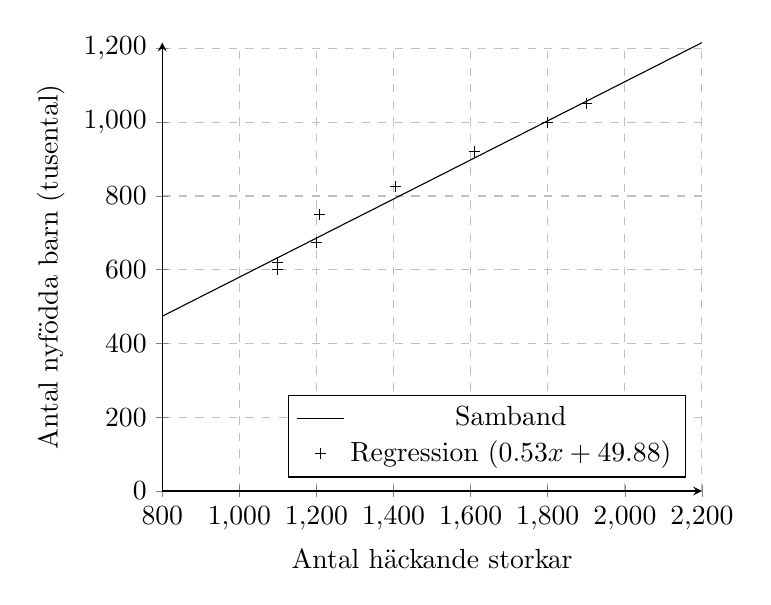
\begin{tikzpicture}
	\begin{axis}[
			xlabel=Antal häckande storkar,
			ylabel=Antal nyfödda barn (tusental),
			axis lines = left,
			legend pos=south east,
			grid style=dashed,
			ymajorgrids=true,
			xmajorgrids=true,
			domain={current axis.above origin:1900},
			ymin=0,
			legend entries={Samband, Regression ($0.53x+49.88$)}
			]
			\addplot[domain=800:2200,no markers]{0.53*x+49.88};
			\addplot[only marks,mark=+] coordinates {
				(1900,1050)
				(1800,1000)
				(1610,920)
				(1405,825)
				(1208,750)
				(1200,675)
				(1100,620)
				(1100,600)
			};
	\end{axis}
\end{tikzpicture}
